\chapter{System Analysis and Architecture}

\section{Functional Overview of the System}

VoidLink is a secure messaging system that enables users to exchange encrypted messages through a centralized server that cannot decrypt the content. The system implements a complete messaging lifecycle from user registration through message delivery, with cryptographic security enforced at every step.

\subsection{Core Functional Requirements}

\textbf{User Management:}
\begin{itemize}
    \item Account registration with username and password
    \item Cryptographic key pair generation (Ed25519)
    \item Encrypted private key backup with user-chosen passphrase
    \item Multi-device support through cloud key backup
    \item Account session management with 24-hour expiration
\end{itemize}

\textbf{Contact Management:}
\begin{itemize}
    \item Contact request sending with optional message
    \item Contact request acceptance or rejection
    \item Mutual contact relationship enforcement
    \item Contact list with online presence indicators
    \item Public key retrieval for encryption
\end{itemize}

\textbf{Messaging:}
\begin{itemize}
    \item End-to-end encrypted message sending
    \item Real-time message delivery via WebSocket
    \item Offline message queuing with automatic delivery
    \item Message delivery and read confirmations
    \item Typing indicators for active conversations
    \item Message history retrieval with pagination
\end{itemize}

\textbf{Security:}
\begin{itemize}
    \item Two-layer authentication (account + cryptographic)
    \item Challenge-response authentication using Ed25519 signatures
    \item Cryptographic session management with 15-minute expiration
    \item Comprehensive audit logging of security events
    \item Rate limiting on authentication endpoints
\end{itemize}

\section{Actors and Interactions}

\subsection{System Actors}

\textbf{End User:}
\begin{itemize}
    \item Registers account and generates cryptographic keys
    \item Sends and receives encrypted messages
    \item Manages contact relationships
    \item Verifies correspondent identities through key fingerprints
\end{itemize}

\textbf{Client Application (Browser):}
\begin{itemize}
    \item Performs all cryptographic operations
    \item Manages private keys in memory and encrypted storage
    \item Encrypts messages before transmission
    \item Decrypts received messages for display
    \item Maintains WebSocket connection for real-time updates
\end{itemize}

\textbf{Backend Server:}
\begin{itemize}
    \item Authenticates users through two-layer system
    \item Routes encrypted messages between users
    \item Stores encrypted payloads without decryption capability
    \item Manages message queue for offline delivery
    \item Tracks user presence and connection status
    \item Logs security events for audit purposes
\end{itemize}

\textbf{Database:}
\begin{itemize}
    \item Stores account credentials (hashed passwords)
    \item Stores public keys and encrypted private key backups
    \item Stores encrypted message payloads
    \item Stores contact relationships and metadata
    \item Stores session tokens and authentication challenges
\end{itemize}

\subsection{Actor Interactions}

The system enforces strict interaction patterns to maintain security:

\begin{enumerate}
    \item User interacts only with Client Application
    \item Client Application performs cryptographic operations locally
    \item Client Application communicates with Backend Server via HTTPS/WebSocket
    \item Backend Server validates authentication but never accesses plaintext
    \item Backend Server stores and retrieves encrypted data from Database
    \item Database stores opaque encrypted blobs without interpretation
\end{enumerate}

\section{Global Architecture}

\subsection{Trust Boundary Model}

VoidLink's architecture is defined by a clear trust boundary:

\textbf{Trusted Zone (Client-Side):}
\begin{itemize}
    \item User's web browser environment
    \item JavaScript cryptographic libraries (TweetNaCl.js)
    \item Private keys in memory during active session
    \item Encrypted private keys in browser localStorage
    \item User interface and application logic
\end{itemize}

\textbf{Untrusted Zone (Server-Side):}
\begin{itemize}
    \item Backend server application
    \item Database storage
    \item Network infrastructure
    \item System administrators
    \item Any third-party with server access
\end{itemize}

\textbf{Trust Boundary Enforcement:}
\begin{itemize}
    \item Private keys never cross the trust boundary unencrypted
    \item All encryption/decryption occurs in trusted zone
    \item Server receives only encrypted payloads
    \item Cryptographic authentication proves key possession without revealing keys
\end{itemize}

\subsection{Component Architecture}

The system consists of three main architectural layers:

\textbf{Presentation Layer (Frontend):}
\begin{itemize}
    \item React components for user interface
    \item Zustand stores for state management
    \item Crypto services for key management and encryption
    \item WebSocket client for real-time communication
    \item API client for REST operations
\end{itemize}

\textbf{Application Layer (Backend):}
\begin{itemize}
    \item Express REST API routes
    \item WebSocket server for real-time messaging
    \item Authentication middleware (two-layer)
    \item Message queue service for offline delivery
    \item Connection manager for presence tracking
\end{itemize}

\textbf{Data Layer (Database):}
\begin{itemize}
    \item PostgreSQL relational database
    \item 10 tables for accounts, sessions, messages, contacts
    \item Helper functions for contact validation
    \item Indexes for query optimization
    \item Audit event storage
\end{itemize}

\begin{figure}[H]
    \centering
    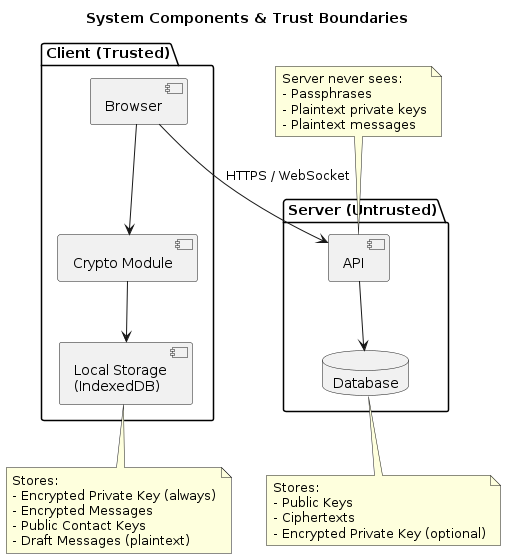
\includegraphics[width=0.9\textwidth]{../diagram/component diagram.png}
    \caption{VoidLink Component Architecture Diagram}
    \label{fig:component-diagram}
\end{figure}

\section{Frontend / Backend Separation}

\subsection{Frontend Responsibilities}

The frontend (trusted zone) handles all security-critical operations:

\textbf{Cryptographic Operations:}
\begin{itemize}
    \item Key pair generation using TweetNaCl.js
    \item Message encryption with NaCl box (Curve25519 + XSalsa20 + Poly1305)
    \item Message decryption for display
    \item Challenge signing with Ed25519
    \item Private key encryption with user passphrase
\end{itemize}

\textbf{Key Management:}
\begin{itemize}
    \item Secure random key generation
    \item Private key storage in encrypted form
    \item Session-based private key caching
    \item Key derivation (Ed25519 to Curve25519)
    \item Key fingerprint generation for verification
\end{itemize}

\textbf{State Management:}
\begin{itemize}
    \item Authentication state (account and crypto tokens)
    \item Contact list with public keys
    \item Message history with decrypted content
    \item Active conversation tracking
    \item User presence and typing indicators
\end{itemize}

\subsection{Backend Responsibilities}

The backend (untrusted zone) provides infrastructure without accessing plaintext:

\textbf{Account Management:}
\begin{itemize}
    \item User registration with password hashing (bcrypt)
    \item Account session creation and validation
    \item Session token generation and expiration
    \item Account status management
\end{itemize}

\textbf{Cryptographic Authentication:}
\begin{itemize}
    \item Challenge generation (random 32-byte values)
    \item Signature verification using stored public keys
    \item Crypto session creation and validation
    \item Challenge expiration and cleanup
\end{itemize}

\textbf{Message Routing:}
\begin{itemize}
    \item Encrypted payload storage
    \item Message delivery via WebSocket
    \item Offline message queuing
    \item Delivery confirmation tracking
\end{itemize}

\textbf{Contact Management:}
\begin{itemize}
    \item Contact request storage and notification
    \item Mutual relationship enforcement
    \item Contact list retrieval with presence data
    \item Public key distribution
\end{itemize}

\subsection{Communication Protocol}

\textbf{REST API (HTTPS):}
\begin{itemize}
    \item Account operations (register, login, logout)
    \item Crypto operations (upload key, challenge, verify)
    \item Contact operations (request, accept, list)
    \item Message operations (send, history, delivery)
\end{itemize}

\textbf{WebSocket Protocol:}
\begin{itemize}
    \item Real-time message delivery
    \item Presence updates (online/offline)
    \item Typing indicators
    \item Delivery and read confirmations
    \item Contact request notifications
\end{itemize}

\section{Authentication Flow Overview}

\subsection{Two-Layer Authentication Model}

VoidLink implements a unique two-layer authentication system:

\textbf{Layer 1: Account Authentication}
\begin{itemize}
    \item Purpose: Account access and management
    \item Method: Username/password with bcrypt hashing
    \item Session Duration: 24 hours
    \item Token: Account session token (64-character hex)
    \item Scope: Account operations, key management, settings
\end{itemize}

\textbf{Layer 2: Cryptographic Authentication}
\begin{itemize}
    \item Purpose: Message operations and cryptographic actions
    \item Method: Ed25519 challenge-response signature
    \item Session Duration: 15 minutes (sliding window)
    \item Token: Crypto session token (64-character hex)
    \item Scope: Message sending/receiving, contact operations
\end{itemize}

\subsection{Registration and Initial Setup Flow}

\begin{enumerate}
    \item User provides username, password, and passphrase
    \item Client generates Ed25519 key pair locally
    \item Client encrypts private key with passphrase using NaCl secretbox
    \item Client sends registration request with username and password
    \item Server creates account with hashed password (bcrypt, cost 12)
    \item Client receives account session token
    \item Client uploads public key to server
    \item Client uploads encrypted private key backup to server
    \item Client completes crypto challenge to obtain crypto session token
    \item User is fully authenticated and can send messages
\end{enumerate}

\begin{figure}[H]
    \centering
    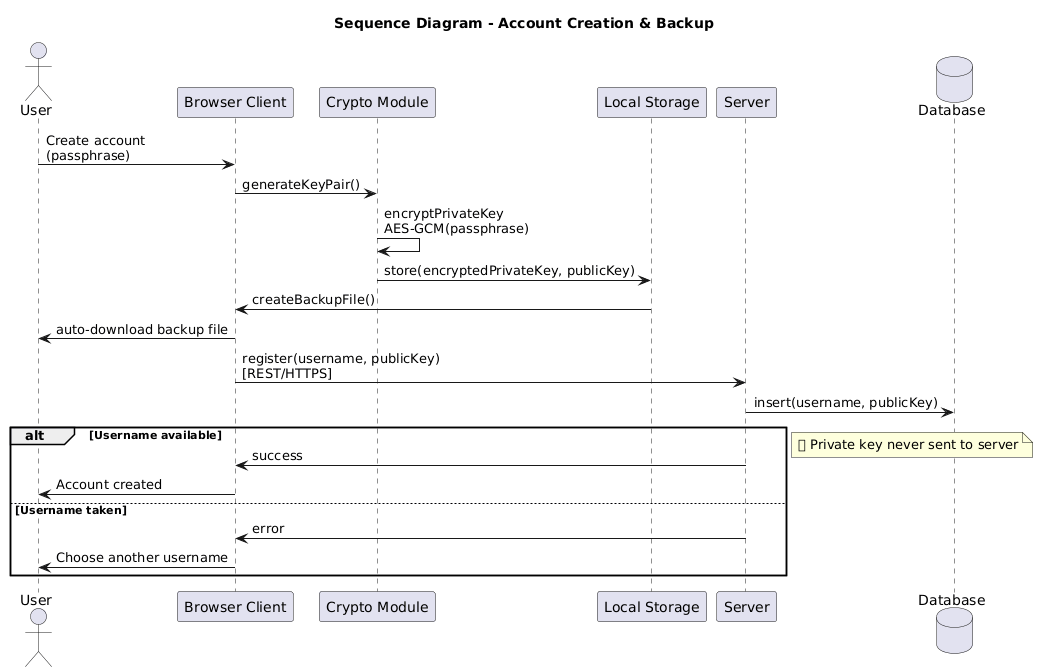
\includegraphics[width=0.9\textwidth]{../diagram/sequence_diagram_account_creation_backup.png}
    \caption{Account Creation and Backup Sequence Diagram}
    \label{fig:account-creation}
\end{figure}

\subsection{Login Flow}

\begin{enumerate}
    \item User provides username, password, and passphrase
    \item Client sends login request to server
    \item Server validates credentials and returns account session token
    \item Client attempts to decrypt local encrypted private key with passphrase
    \item If local key unavailable, client fetches encrypted backup from server
    \item Client decrypts private key with passphrase
    \item Client requests crypto challenge from server
    \item Server generates random 32-byte challenge
    \item Client signs challenge with private key (Ed25519)
    \item Client sends signed challenge to server
    \item Server verifies signature using stored public key
    \item Server returns crypto session token
    \item User is authenticated and can send messages
\end{enumerate}

\begin{figure}[H]
    \centering
    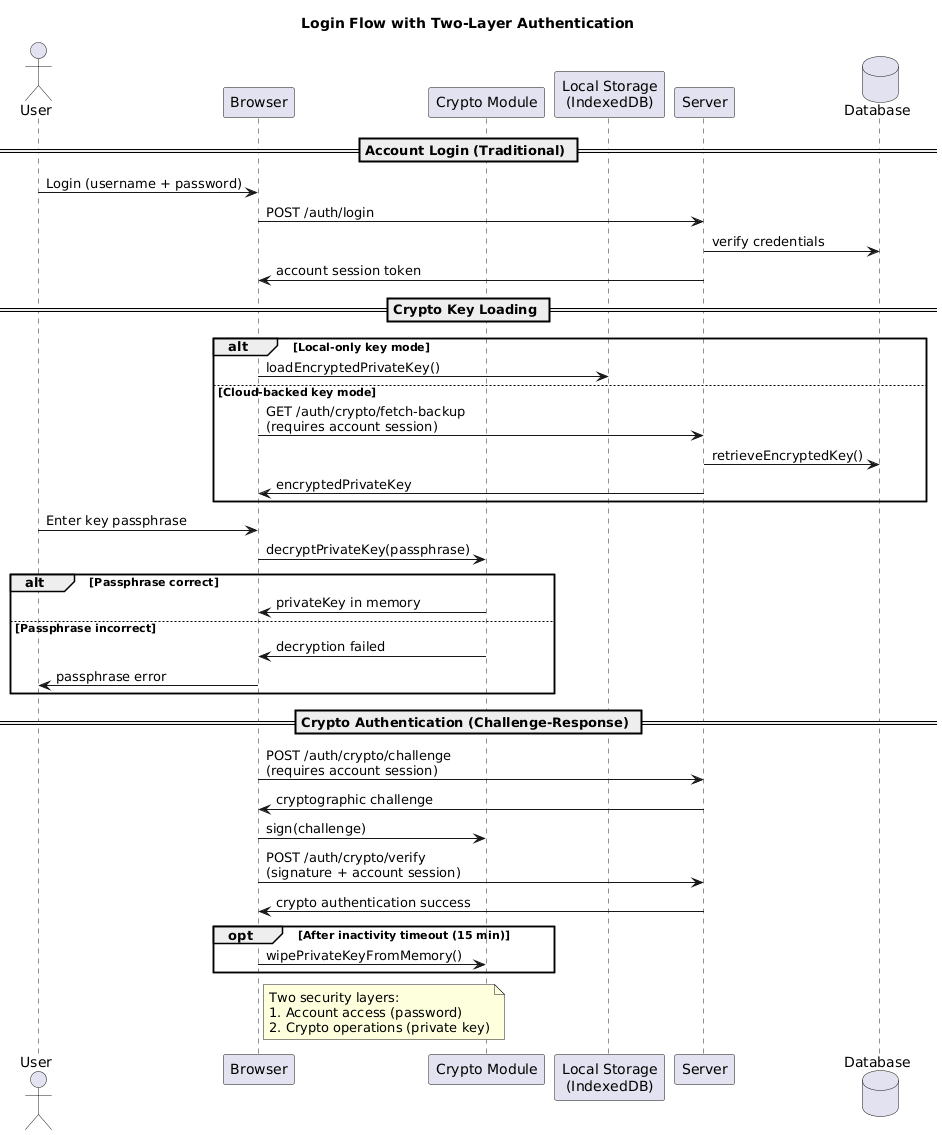
\includegraphics[width=0.9\textwidth]{../diagram/sequence_diagram_login_auth.png}
    \caption{Login and Authentication Sequence Diagram}
    \label{fig:login-auth}
\end{figure}

\subsection{Session Management}

\textbf{Account Session:}
\begin{itemize}
    \item Created on successful login
    \item Stored in database with expiration timestamp
    \item Includes IP address and user agent for audit
    \item Validated on every API request
    \item Automatically cleaned up after expiration
\end{itemize}

\textbf{Crypto Session:}
\begin{itemize}
    \item Created after successful challenge verification
    \item Linked to parent account session (cascading delete)
    \item Required for all message operations
    \item Shorter expiration for increased security
    \item Sliding window extends on activity
\end{itemize}

\section{Secure Messaging Flow Overview}

\subsection{Message Encryption Process}

\begin{enumerate}
    \item User composes message in client interface
    \item Client retrieves recipient's public key from contact list
    \item Client converts Ed25519 keys to Curve25519 format
    \item Client generates random 24-byte nonce
    \item Client encrypts message using NaCl box:
    \begin{itemize}
        \item Authenticated encryption (Curve25519-XSalsa20-Poly1305)
        \item Combines sender's private key and recipient's public key
        \item Produces ciphertext with authentication tag
    \end{itemize}
    \item Client creates JSON payload: \{nonce, encrypted\}
    \item Client sends encrypted payload to server via WebSocket
    \item Server stores encrypted payload without decryption
    \item Server routes message to recipient if online
    \item Server queues message if recipient offline
\end{enumerate}

\subsection{Message Decryption Process}

\begin{enumerate}
    \item Client receives encrypted payload via WebSocket
    \item Client identifies sender from message metadata
    \item Client retrieves sender's public key from contact list
    \item Client retrieves own private key from session memory
    \item Client converts Ed25519 keys to Curve25519 format
    \item Client extracts nonce and ciphertext from payload
    \item Client decrypts using NaCl box.open:
    \begin{itemize}
        \item Combines own private key and sender's public key
        \item Verifies authentication tag
        \item Decrypts ciphertext to plaintext
    \end{itemize}
    \item Client displays decrypted message to user
    \item Client sends delivery confirmation to server
    \item Client sends read confirmation if conversation is active
\end{enumerate}

\begin{figure}[H]
    \centering
    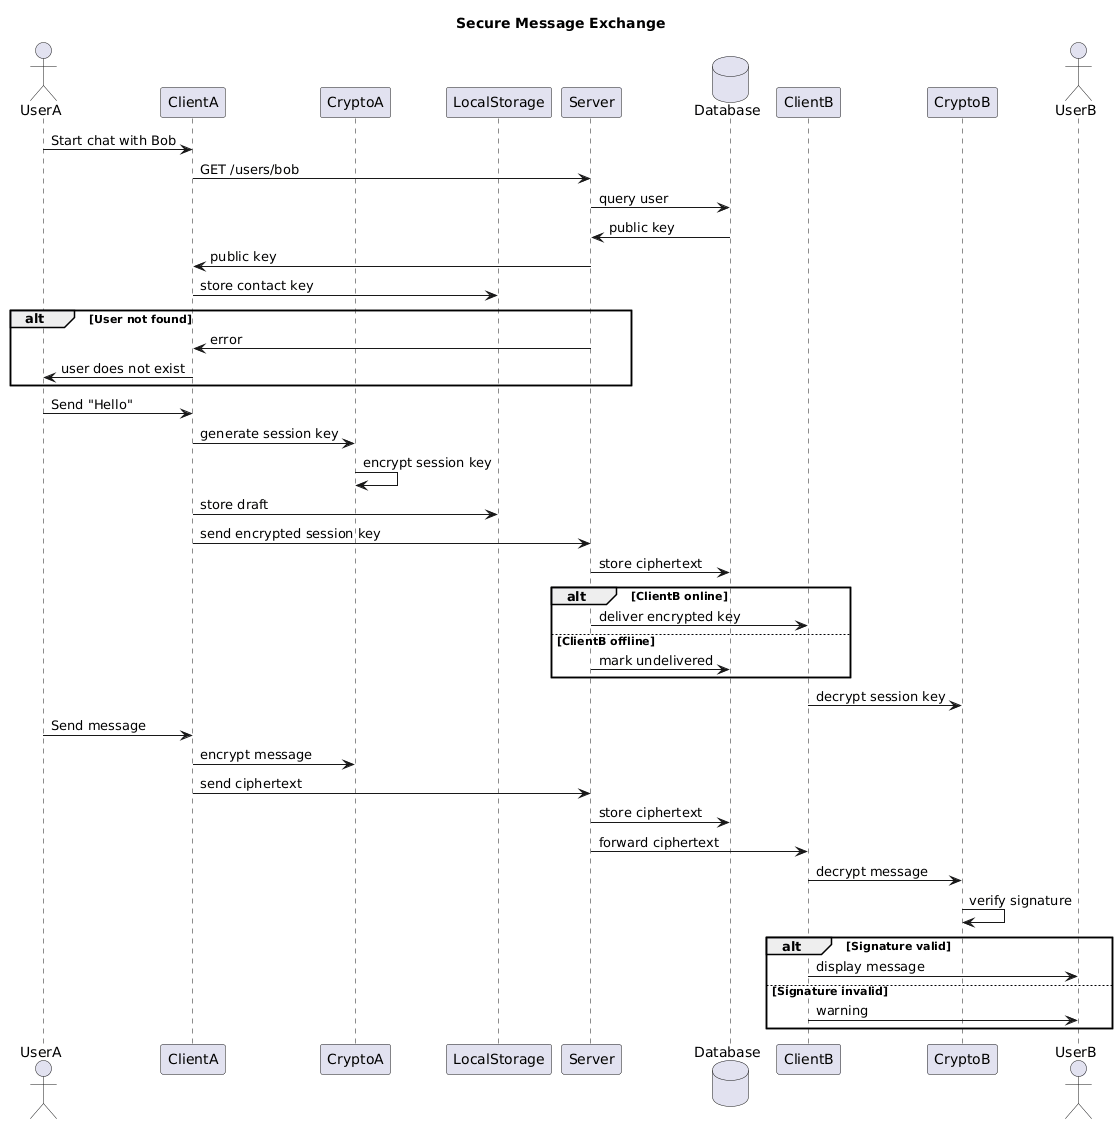
\includegraphics[width=0.9\textwidth]{../diagram/sequence_diagram_secure_messageex.png}
    \caption{Secure Message Exchange Sequence Diagram}
    \label{fig:message-exchange}
\end{figure}

\subsection{Offline Message Delivery}

\begin{enumerate}
    \item Sender sends message while recipient is offline
    \item Server detects recipient is not connected
    \item Server stores message in message\_queue table
    \item Server marks message with priority and timestamp
    \item Recipient comes online and establishes WebSocket connection
    \item Server detects recipient connection
    \item Message queue service retrieves queued messages
    \item Server delivers queued messages via WebSocket
    \item Client decrypts and displays messages
    \item Server marks messages as delivered in queue
    \item Server cleans up processed queue entries after 24 hours
\end{enumerate}

\subsection{Real-Time Features}

\textbf{Presence Tracking:}
\begin{itemize}
    \item WebSocket connection establishes user as online
    \item Server increments connection count in user\_presence table
    \item Server broadcasts presence update to user's contacts
    \item Client displays online/offline indicators
    \item WebSocket disconnection decrements connection count
    \item User marked offline when connection count reaches zero
\end{itemize}

\textbf{Typing Indicators:}
\begin{itemize}
    \item Client detects typing in message input field
    \item Client sends typing\_start event via WebSocket
    \item Server forwards to recipient if online
    \item Client displays typing indicator for sender
    \item Client sends typing\_stop after 3 seconds of inactivity
    \item Server forwards stop event to recipient
    \item Client removes typing indicator
\end{itemize}

\textbf{Delivery Confirmations:}
\begin{itemize}
    \item Client receives message and decrypts successfully
    \item Client sends message\_delivered event to server
    \item Server updates message.delivered flag in database
    \item Server forwards delivery confirmation to sender
    \item Sender's client updates message status to "delivered"
    \item If recipient has conversation open, client sends message\_read event
    \item Server forwards read confirmation to sender
    \item Sender's client updates message status to "read"
\end{itemize}

\section{Architecture and Sequence Diagrams}

The following diagrams illustrate the system architecture and key operational flows:

\subsection{Component Diagram}

Figure \ref{fig:component-diagram} shows the high-level component architecture, illustrating the separation between trusted (client-side) and untrusted (server-side) zones. The diagram highlights the cryptographic operations performed exclusively in the client and the opaque data handling in the server.

\subsection{Account Creation Sequence}

Figure \ref{fig:account-creation} details the complete account creation and key backup process, showing how private keys are generated client-side, encrypted with a user passphrase, and backed up to the server in encrypted form.

\subsection{Authentication Sequence}

Figure \ref{fig:login-auth} illustrates the two-layer authentication process, showing both the traditional username/password authentication and the cryptographic challenge-response authentication that proves key possession without revealing the private key.

\subsection{Message Exchange Sequence}

Figure \ref{fig:message-exchange} demonstrates the end-to-end encrypted message flow, from encryption in the sender's client through server routing to decryption in the recipient's client, emphasizing that the server never has access to plaintext content.

\subsection{Key Rotation Sequence}

\begin{figure}[H]
    \centering
    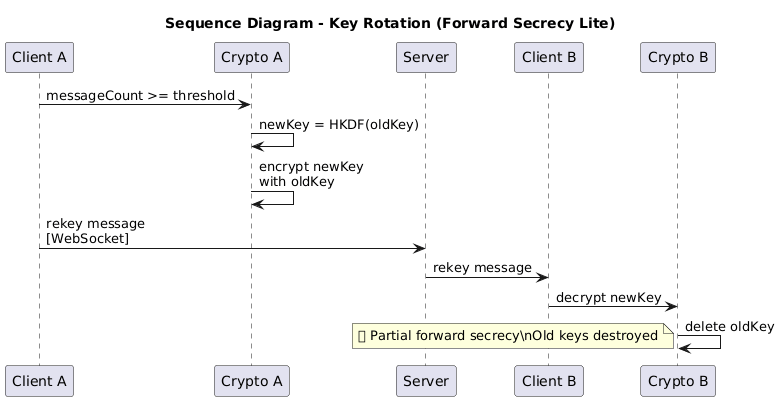
\includegraphics[width=0.9\textwidth]{../diagram/sequence_diagram_key_rotation.png}
    \caption{Key Rotation Sequence Diagram}
    \label{fig:key-rotation}
\end{figure}

Figure \ref{fig:key-rotation} shows the key rotation process, which allows users to generate new key pairs while maintaining message history. This feature is designed but not yet implemented in the current version.

\subsection{User Flow Activity Diagram}

\begin{figure}[H]
    \centering
    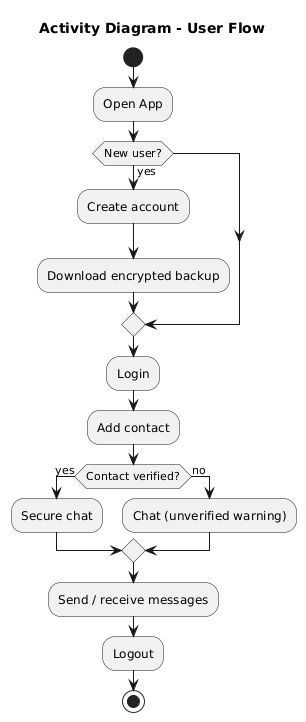
\includegraphics[width=0.8\textwidth]{../diagram/Activity_diagram_user_flow.png}
    \caption{User Flow Activity Diagram}
    \label{fig:user-flow}
\end{figure}

Figure \ref{fig:user-flow} presents the complete user journey from registration through messaging, showing decision points and alternative flows for different scenarios.
\end{document}
